Lors du lancement du jeu, les utilisateurs accèderont au menu d'accueil

\begin{figure}[H]
    \centering
    
\includegraphics[width=0.8\textwidth ]{images/startingPage/start.png}
    \caption{Menu d'acceuil}
    \label{fig:pic_dessus}
\end{figure}

Depuis ce menu, un utilisateur peut soit accéder aux paramètres du jeu en cliquant sur \textbf{config}, soit lancer directement le jeu en cliquant sur \textbf{play}.

Si l'utilisateur lance directement le jeu, il sera redirigé sur la carte du village :

\begin{figure}[H]
    \centering
    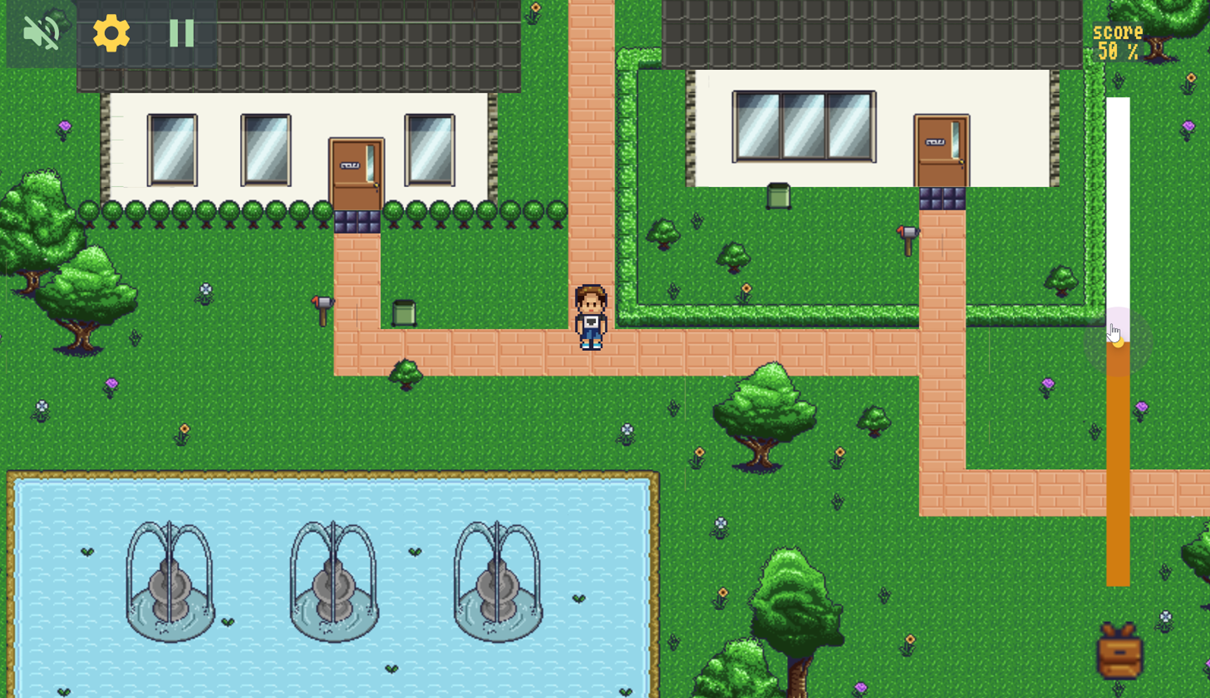
\includegraphics[width=0.8\textwidth ]{images/startingPage/village1.png}
    \caption{Village}
    \label{fig:pic_dessus}
\end{figure}

Dans le cas où l'utilisateur souhaiterait modifier les paramètres, il sera d'abord redirigé sur cette page avant de pouvoir lancer le jeu :
\begin{figure}[H]
    \centering
    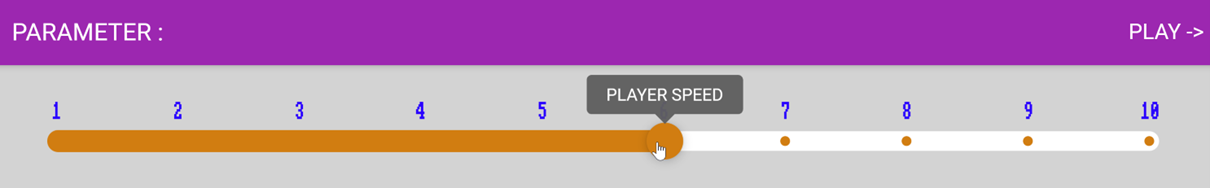
\includegraphics[width=0.8\textwidth ]{images/startingPage/setting.png}
    \caption{Paramètres}
    \label{fig:pic_dessus}
\end{figure}